\section*{Dati e risultati}

\subsection*{Registro a scorrimento}

In questa sezione della nostra esperienza vogliamo realizzare un registro a scorrimento con ricircolo. Per realizzare tale circuito ci serviamo di due circuiti integrato SN74LS109, quindi di 4 flip-flop di tipo JK. Il circuito che abbiamo realizzato è riportato in Figura \ref{fig:registro}.
La modalità di funzionamento di tale dispositivo è la segunte: i flip-flop JK vengono utilizzati in modalità D, ovvero sfruttano il ritardo nella propagazione del segnale dovuta alle capacità parassite interne al dispositivo.
Quindi andiamo ad alimentare il circuito con una tensione $V\ped{cc}^+\,=\,\SI{+5}{\volt}$ ed una $V\ped{cc}^-\,=\,\SI{0}{\volt}$, inoltre poniamo come segnale di clock un'onda quadra di frequenza a piacere di ampiezza picco picco \SI{5}{\volt} e con una tensione di offset di \SI{+2.5}{\volt}.
Quindi possiamo notare, aiutandoci dalla Figura \ref{fig:registro}, che il segnale di clock è comune atutti e quattro i flip-flop. In questo modo, sfruttando le linee di Preset e Clear io memorizzo in fase di accensione un 1 logico nel primo flip-flop e uno 0 in tutti gli altri. Sucessivamente, grazie al segnale di clock l'uno logico si sposta man mano da sinistra a destra passando da un flip-flop a quellosuccessivo ogni fronte in salita dell'impulso di clock. Infine possiamo notare che, dal momento che l'uscita dell'ultimo flip-flop e riportata in ingresso al primo flip-flop, l'uno logico cicla all'infinito. In questo modo collegando alle quatro uscite la schedina LED possiamo effettivamente osservare l'accensione del led corrispondente all'uscita che si trova ad 1 logico.
Idealmente abbiamo riprodotto ad esempio una ila di luci ad intermittenza che vengono utilizzate negli aereoporti per segnalare la pista di atterraggio.

\subsection*{Contatore binario}

In questa sezione della relazione vogliamo realizzare un contatore binario. A tal fine abbiamo deciso di sfruttare due circuiti integrati SN74LS191 e un circuito integrato SN74LS109. Abbiamo quindi realizzato il circuito illustrato in Figura \ref{fig:contatore}.
Grazie all'aiuto del datasheet relativo all'integrato SN74LS191 è sappiamo che i flip-flop sono posti in configurazione master-slave e sono sincronizzati sul fronte di salita del segnale di clock. Questo dispositivo può esguire il conteggio sia in avanti (UP) che in dietro (DOWN) a seconda del valore logico presente sull'ingresso di controllo U/D. E` imoprtante ricordare che che la linea di U/D deve cambiare stato logico solo quando il segnale di clock è ad 1 logico, quindi alto.
Sempre razie all'utilizzo del datasheet sappiamo che:
\begin{itemize} \itemsep2pt \parskip0pt \parsep0pt
	\item{La linea in input di Count Enable (CE) è quella che permette di gestire il prestito/riporto in contatori a più stadi in cascata;}
	\item{Le linee di uscita ``TerminalCount'' (TC) (Max/min) e ``RippleClock'' (RC) permettono di indicare una situazione di overflow/underflow del contatore e consentono di scegliere vari metodi per gestire i prestiti/riporti in contatori a più stadi;}
	\item{Il TerminalCount (TC) (Max/min) è normalmente a 0 logico e va ad 1 logico quando il contatore raggiunge il valore zero in count-down oppure il valore massimo pari a 15 in count-up. Il segnale TC è anche usato all’interno del contatore per abilitare il segnale di uscita RippleClock (RC);}
	\item{L’uscita RippleClock (RC) è normalmente ad 1 logico. Quando l’ingresso CE è basso e TC è alto l’uscita RC va a 0 e vi rimane fino a quando il segnale di clock ritorna nuovamente alto;}
\end{itemize}

Quindi, collegando le varie uscite dei diversi flip-flop presenti sul circuito integrato alla schedina LED, siamo in grado di contare effettivamente i cicli di clock in input al nostro circuito. Naturalmente, avendo a disposizione in totale otto flip-flop possiamo contare fino a 15, ricordandoci infatti che i flip-flop a disposizione sono 8 e si parte da 0.
Ricordandoci che un flip-flop JK modifica il suo stato di uscita quando il fronte di clock è in salita, e non lo altera fino ad un nuovo fronte in salita dello stesso segnale.
Quindi che affinchè un flip-flop possa enrare in funzione deve ricevere un segnale da quello precedente, che lo abilita al conteggio. Questo segnale non è altro che l'uscita del flip-flop precedente.

Ricordiamo che il segnale di clock è un'onda quadra di ampiezza \SI{5}{\volt} picco picco con una tensione di offset di \SI{+2.5}{\volt} e una frequenza a piacere, in base alla velocità con cui si vuole contare il segnale di clock. Naturalmente se la frequenza è troppo alta l'occhio umano non riesce a seguire i LED che si illuminano.

\subsection*{Convertitore analogico-digitale.}

In quest'ultima sezione di questa relazione vogliamo realizare un contatore a 8 bit. A tal fine sfruttiamo il circuito realizzato in precedenza, Figura \ref{fig:contatore}, e usando l'intgrato DAC08, al quale colleghiamo le uscite dei flip-flop visti nella sezione sopra, otteniamo il circuito illustarto in Figura \ref{fig:convertitore}.

Per comprendere al meglio il funzionamento del circuito che abbiamo realizzato dobbiamo prima capire come lavora un DAC08. Quindi iniziamo col dire che il DAC08 è un convertitore ad 8 bit in cui l'uscita è il prodotto di un numero digitale per il valore della corrente di riferimento.
Quindi definiamo le seguenti gandezze: $I\ped{ref}$ corrente di riferimento i cui valori normalmente sono compresi tra \SI{0.2}{\milli\ampere} e \SI{4}{\milli\ampere}, $I\ped{14}\,=\,I\ped{ref}$ la corrente sul pin 14 e $I\ped{fr}$ la corrente di uscita (Full Scale).
Ricordiamo la relazione che lega la corrente $I\ped{fr}$ con $I\ped{ref}$:

\begin{equation}
	I\ped{ref}\,=\,\frac{255}{256} \cdot I\ped{ref}
	\label{eq:corrente}
\end{equation}

A questo punto abbiamo usato l'alimentatore per alimentare il DAC08 a tensioni di +15 e -15 \si{\volt} e per fornire la tensione di riferimento $V\ped{ref}\,=\,\SI{+4}{\volt}$. Sucessivamente abbiamo alimentato la logica TTL con una tensione di \SI{+5}{\volt}. Inoltre abbiamo regolato la tensione di riferimento $V\ped{ref}$ affinchè la corrente di riferimento sia pari a circa \SI{2}{\milli\ampere}.
Infine per verificare il corretto funzionamento del nostro dispositivo abbiamo collegato l'uscita del circuito con l'oscilloscopio.
Quello che abbiamo otenuto è riportato nel grafico in Figura \ref{fig:converter_plot}

Come possiamo notare da quanto ricavato dal grafico in Figura \ref{fig:converter_plot} il segnale in uscita è un dente di sega a scalini. Piu precisamente gli scalini sono equivalenti al valore di tensione in ingresso del circuito. Possiamo vedere che operando con un circuito ad 8 bit, è possibile contare fino a 256. Questo fatto si può verificare prendendo la tensione massima dell'onda a dente di sega e dividendola per l'altezza di uno scalino...



%\begin{wrapfloat}{table}{I}{300pt}
%\centering
%	\begin{tabular}{l | llll | l}
%	\toprule
%		In & A & B & C & D & Out\\
%	\midrule
%		1 & 0 & 1 & 0 & 1 & 1 \\
%		0 & 1 & 0 & 1 & 0 & 1 \\
%	\bottomrule
%	\end{tabular}
%	\caption{Tabella di verità del circuito in Figura \ref{fig:ritardo}}
%	\label{tab:ritardo}
%\end{wrapfloat}

%\begin{wrapfloat}{figure}{I}{0pt}
%\includegraphics[width=0.5\textwidth]{Relativo}
%\caption{Esempio di figura ‘‘avvolta’’ da un testo.}
%\end{wrapfloat}

%\begin{center}
%	\begin{tabular}{lll}
%	\toprule
%		A & B & C \\
%	\midrule
%		& & \\
%		& & \\
%		& & \\
%		& & \\
%	\bottomrule
%	\end{tabular}
%\end{center}

%\begin{figure}[t!]
%    \centering
%    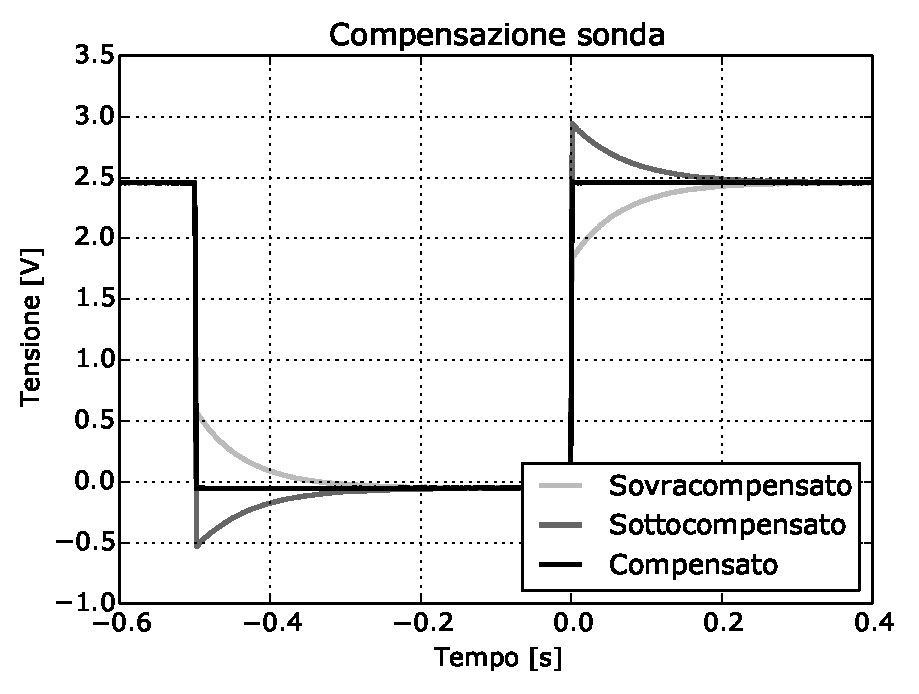
\includegraphics[width=\columnwidth]{figure/comp.pdf}
%    \caption{Input dell'oscilloscopio con una sonda compensabile. Cambiando capacità
%        si può ottenere una sottocompensazione, una sovracompensazione oppure compensare perfettamente
%        le capacità, ottenendo un'onda quadra.}
%    \label{fig:compensazione}
%\end{figure}

%\begin{wrapfloat}{figure}{O}{0pt}
%        \def\svgwidth{0.4\textwidth}
%        \subimport{figure/}{raddrizzatore.pdf_tex}
%        \caption{Raddrizzatore di precisione a semionda. Alimentato, inizialmente con una $V\ped{in}\,=\,\SI{1.02}{\volt}$ di frequenza $\nu\,=\,\SI{50}{\hertz}$.}
%        \label{fig:radd}
%\end{wrapfloat}

%\begin{SCfigure}[][p]
%        \centering
%        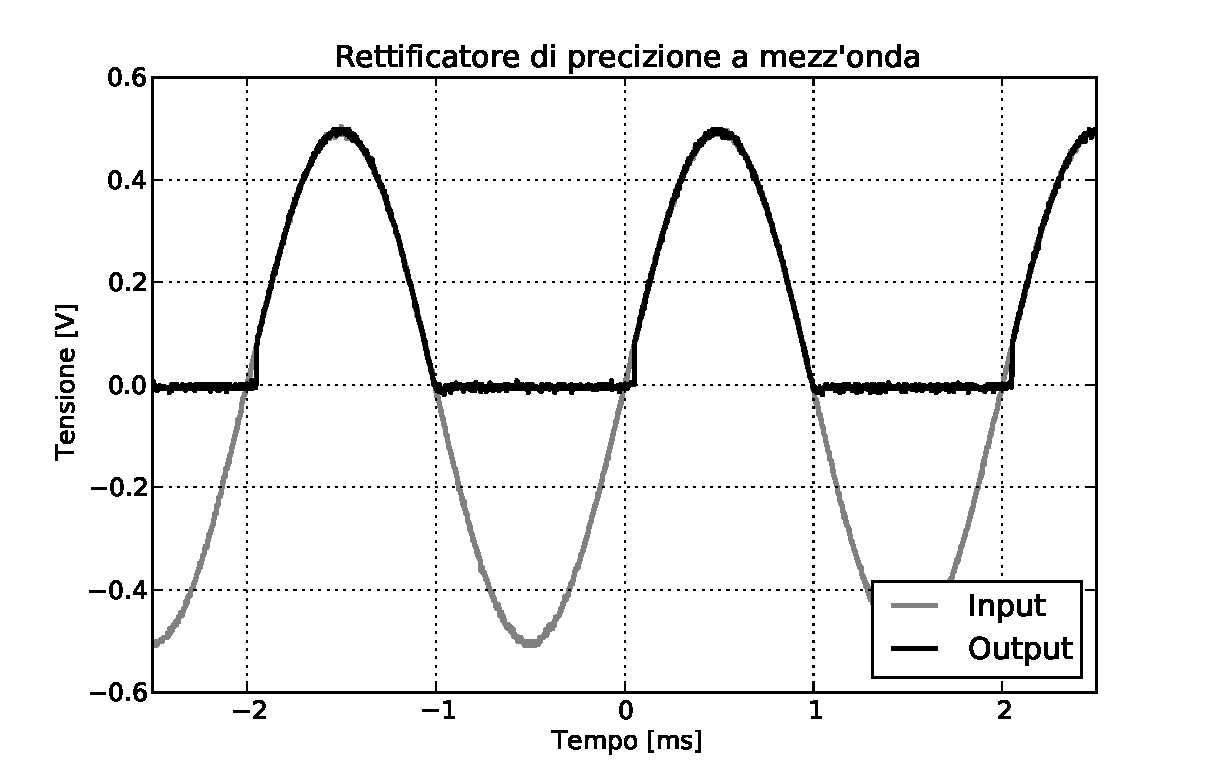
\includegraphics[width=0.7\textwidth]{figure/rett.pdf}
%        \caption{Questo grafico illustra l'andamento di $V\ped{out}$, linea nera, in funzione di $V\ped{in}$, linea grigia. Si nota chiaramente, come da previsioni, che la parte negativa del segnale in ingresso impediscse al diodo di condurre, pertanto la tensione di output risulta nulla. Inoltre, come si può osservare, il fronte di salita di $V\ped{out}$ presenta un leggero ritardo rispetto al segnale in ingresso $V\ped{in}$. Questo ritardo è stato stimato essere approssimativamente di circa $(152\pm10)\SI{}{\micro\second}$.}
%        \label{fig:radd_plot1}
%\end{SCfigure}
